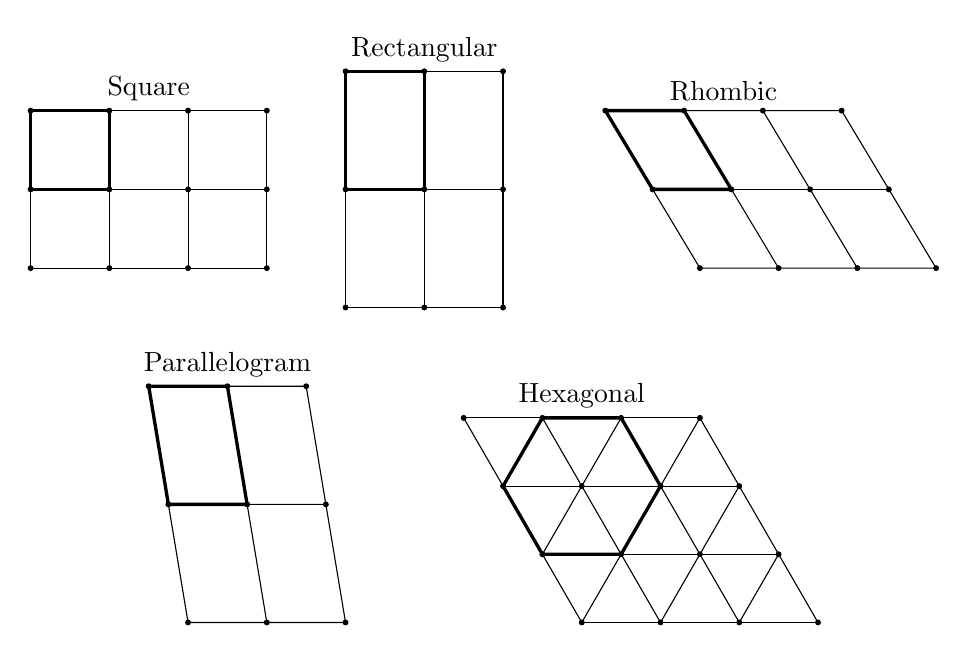
\begin{tikzpicture}[scale=1]

\node [above] at (0,7) {Rectangular};
\draw (-1,4) -- (1,4) -- (1,7) -- (-1,7) -- cycle;
\draw  (0,4) -- (0,7)  (-1,5.5) -- (1,5.5);
\draw [very thick] (-1,5.5) -- (-1,7) -- (0,7) -- (0,5.5) -- cycle;
\foreach \x in {-1,0,1} \filldraw[fill=black, draw=black] (\x,4) circle (0.03);
\foreach \x in {-1,0,1} \filldraw[fill=black, draw=black] (\x,5.5) circle (0.03);
\foreach \x in {-1,0,1} \filldraw[fill=black, draw=black] (\x,7) circle (0.03);

\node [above] at (-3.5,6.5) {Square};
\draw (-2,4.5) -- (-5,4.5) -- (-5,6.5) -- (-2,6.5) -- cycle;
\draw  (-2,5.5) -- (-5,5.5)  (-3,4.5) -- (-3,6.5) (-4,4.5) -- (-4,6.5);
\draw [very thick] (-5,5.5) -- (-5,6.5) -- (-4,6.5) -- (-4,5.5) -- cycle;
\foreach \x in {-2, -3, -4, -5} \filldraw[fill=black, draw=black] (\x,4.5) circle (0.03);
\foreach \x in {-2, -3, -4, -5} \filldraw[fill=black, draw=black] (\x,5.5) circle (0.03);
\foreach \x in {-2, -3, -4, -5} \filldraw[fill=black, draw=black] (\x,6.5) circle (0.03);

\node [above] at (3.8,6.5) {Rhombic};
\draw (3.5,4.5)   -- (6.5,4.5) -- (5.3,6.5) -- (2.3,6.5) -- cycle;
\draw (2.9,5.5) -- (5.9,5.5);
\draw (4.5,4.5) -- (3.3,6.5);
\draw  (5.5,4.5) -- (4.3,6.5);
\draw [very thick] (2.3,6.5) -- (3.3,6.5) -- (3.9,5.5) -- (2.9,5.5) -- cycle;
\foreach \x in {3.5,4.5,5.5,6.5} \filldraw[fill=black, draw=black] (\x,4.5) circle (0.03);
\foreach \x in {2.9,3.9,4.9,5.9} \filldraw[fill=black, draw=black] (\x,5.5) circle (0.03);
\foreach \x in {2.3,3.3,4.3,5.3} \filldraw[fill=black, draw=black] (\x,6.5) circle (0.03);

\node [above] at (-2.5,3) {Parallelogram};
\draw (-1,0) -- (-3,0) -- (-3.5,3) -- (-1.5,3) -- cycle;
\draw  (-2,0) -- (-2.5,3)  (-3.25,1.5) -- (-1.25,1.5);
\draw [very thick] (-3.25,1.5) -- (-3.5,3) -- (-2.5,3) -- (-2.25,1.5) -- cycle;
\foreach \x in {-1,-2,-3} \filldraw[fill=black, draw=black] (\x,0) circle (0.03);
\foreach \x in {-1.25,-2.25,-3.25} \filldraw[fill=black, draw=black] (\x,1.5) circle (0.03);
\foreach \x in {-1.5,-2.5,-3.5} \filldraw[fill=black, draw=black] (\x,3) circle (0.03);

\node [above] at (2,2.6) {Hexagonal}; <!-- Couldn't figure out an elegant way to do the hexagonal lattice - TWJ 6/14/2010 -->
\draw (2,0) -- (5,0);
\draw (1.5,0.866) -- (4.5,0.866);
\draw (1,1.732) -- (4,1.732);
\draw (0.5,2.598) -- (3.5,2.598);
\draw (2,0) -- (0.5,2.598);
\draw (3,0) -- (1.5,2.598);
\draw (4,0) -- (2.5,2.598);
\draw (5,0) -- (3.5,2.598);
\draw (2,0) -- (3.5,2.598);
\draw (3,0) -- (4,1.732);
\draw (4,0) -- (4.5,0.866);
\draw (1.5,0.866) -- (2.5,2.598);
\draw (1,1.732) -- (1.5,2.598);
\draw [very thick] (1.5,0.866) -- (1,1.732) -- (1.5,2.598) -- (2.5,2.598) -- (3,1.732) --  (2.5,0.866) -- cycle;
\foreach \x in {2,3,4,5} \filldraw[fill=black, draw=black] (\x,0) circle (0.03);
\foreach \x in {1.5,2.5,3.5,4.5} \filldraw[fill=black, draw=black] (\x,0.866) circle (0.03);
\foreach \x in {1,2,3,4} \filldraw[fill=black, draw=black] (\x,1.732) circle (0.03);
\foreach \x in {0.5, 1.5,2.5,3.5} \filldraw[fill=black, draw=black] (\x,2.598) circle (0.03);

\end{tikzpicture}
